% This example is meant to be compiled with lualatex or xelatex
% The theme itself also supports pdflatex
\PassOptionsToPackage{unicode}{hyperref}
\documentclass[aspectratio=1610, 9pt]{beamer}

% Load packages you need here
\usepackage{polyglossia}
\setmainlanguage{german}

\usepackage{csquotes}
    

\usepackage{amsmath}
\usepackage{amssymb}
\usepackage{mathtools}

\usepackage{hyperref}
\usepackage{bookmark}

% load the theme after all packages

\usetheme[]{default}

%\title{\LaTeX-Beamer-Theme der TU~Dortmund}
%\author[M.~Nöthe]{Maximilian Nöthe}
%\institute[Kurzform Lehrstuhl]{Names des Lehrstuhls \\  Name der Fakultät}
%\titlegraphic{\includegraphics[width=0.7\textwidth]{images/tudo-title-2.jpg}}


\begin{document}


{
\setbeamertemplate{navigation symbols}{}
\begin{frame}[plain]
    \makebox[\linewidth]{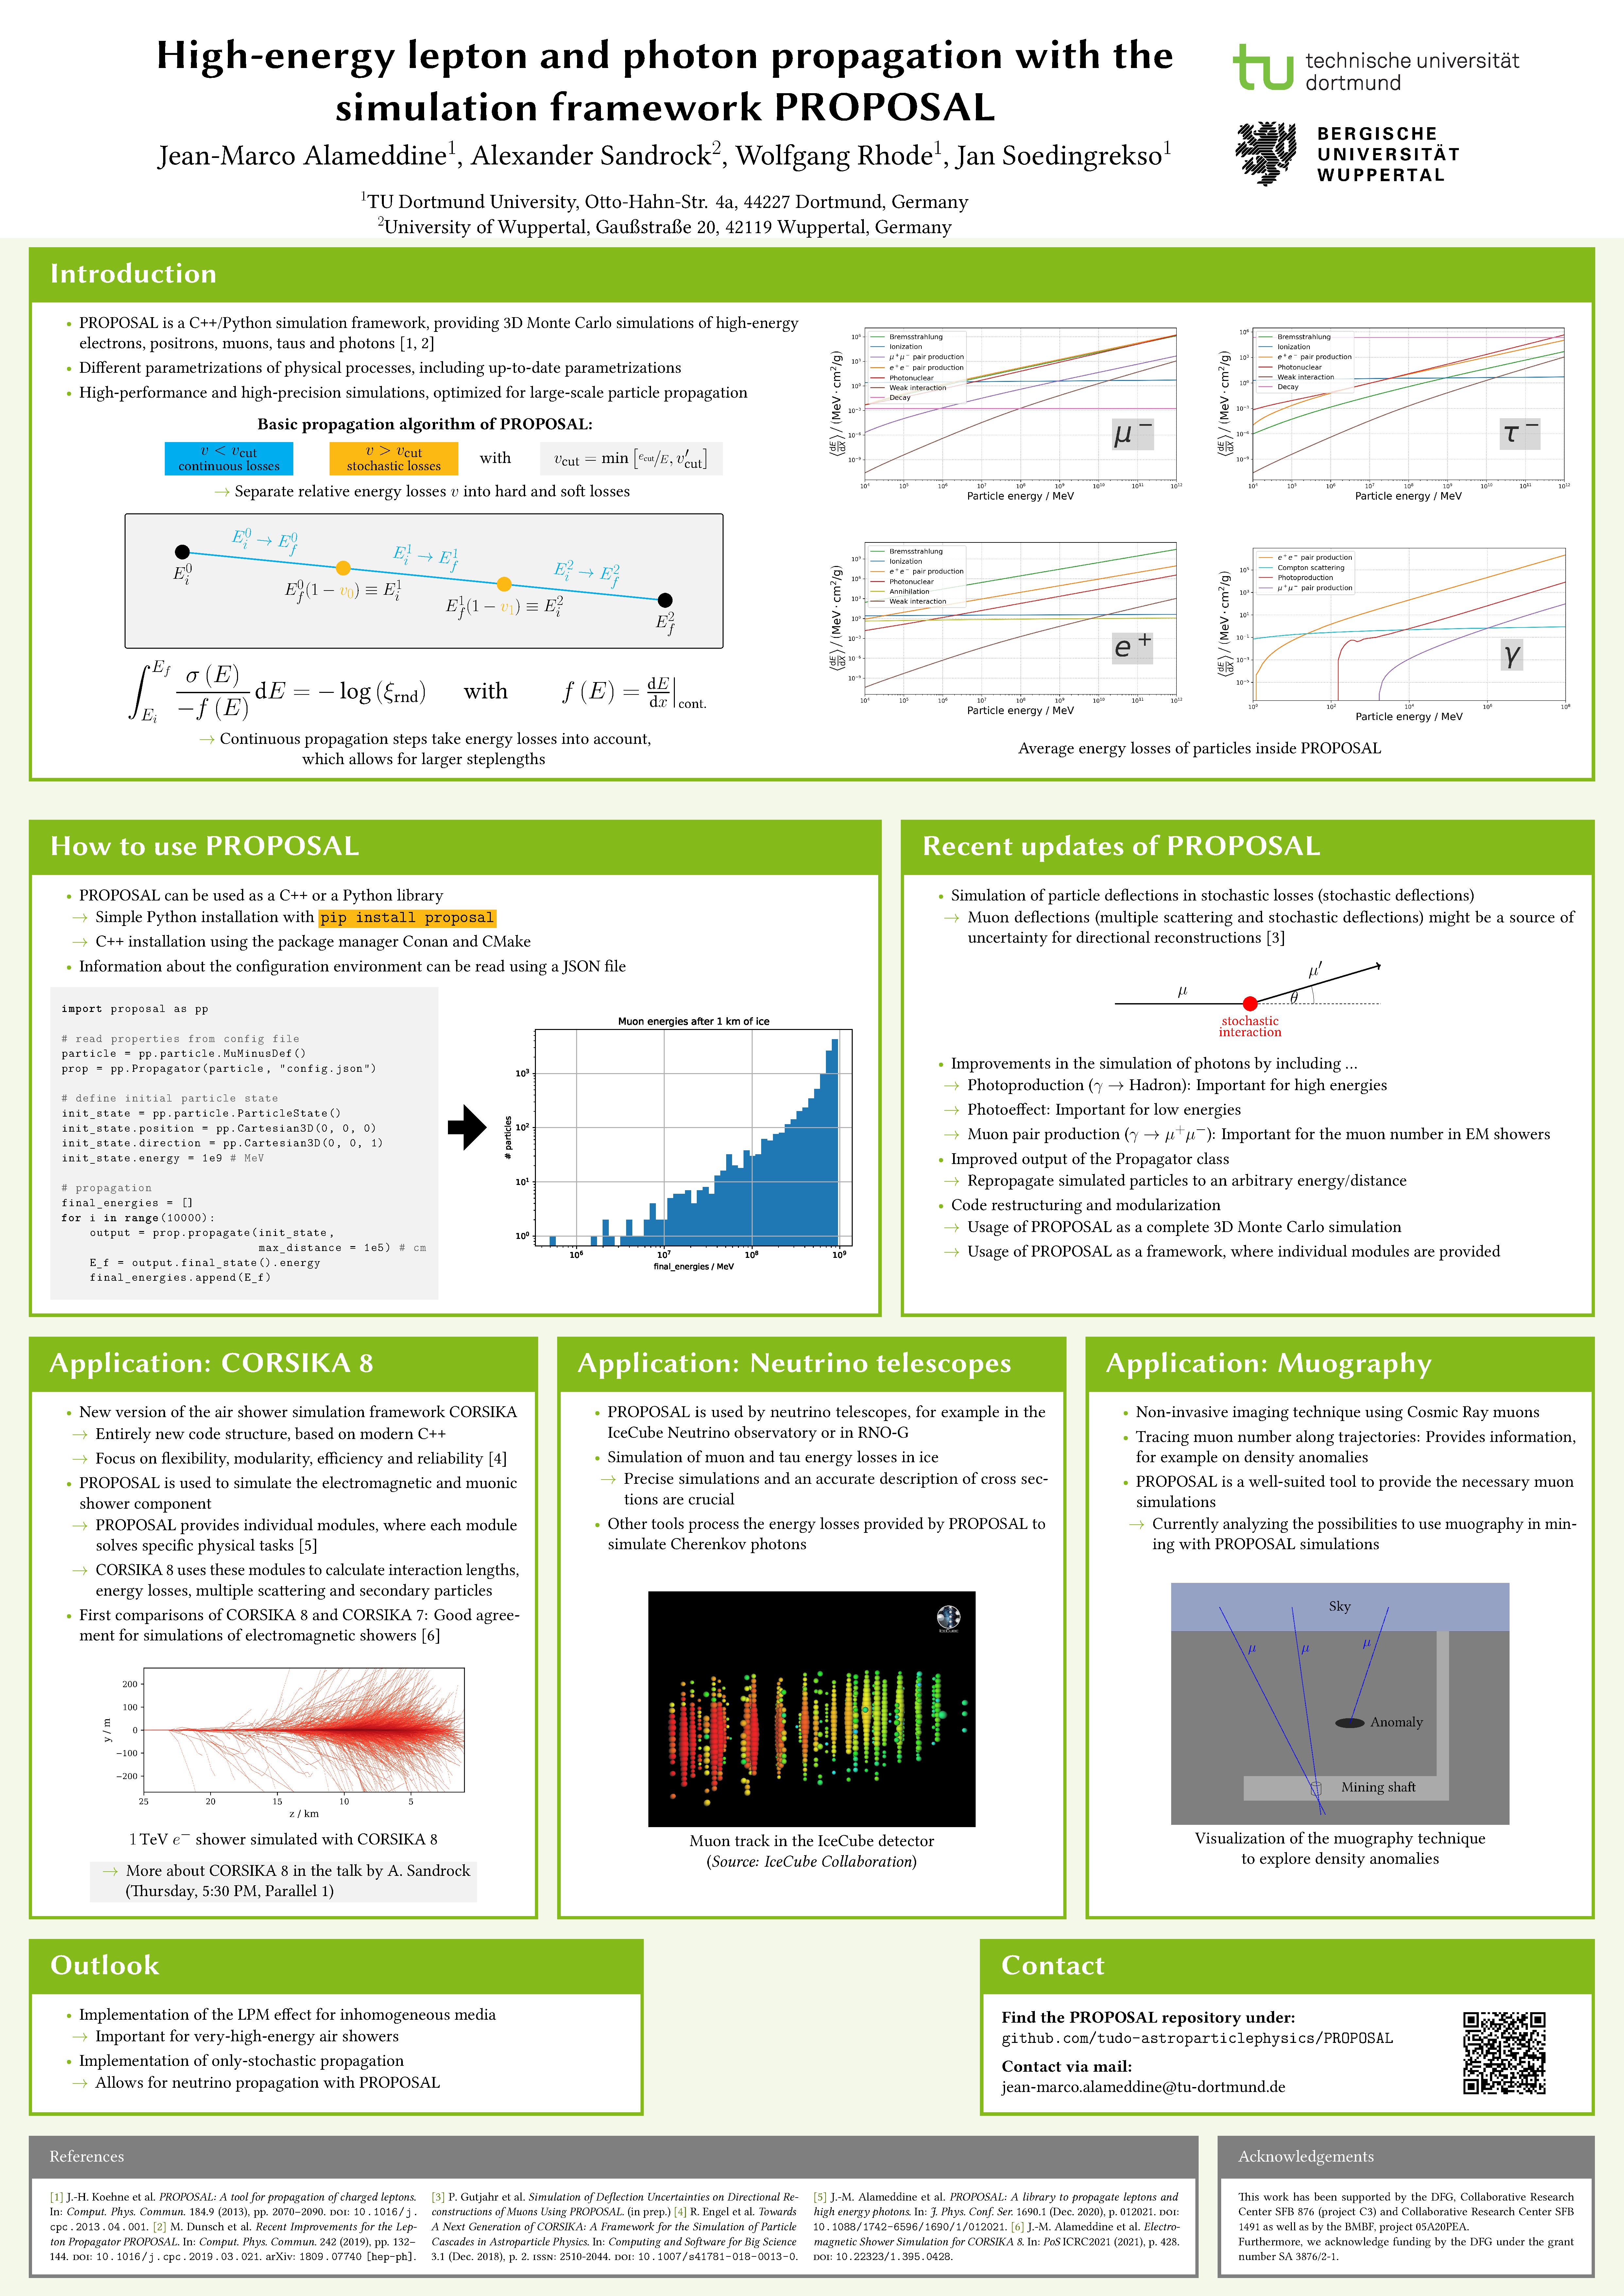
\includegraphics[clip, trim=0cm 0cm 0cm 0cm,height=\paperheight]{../poster_print.pdf}}
\end{frame}
}


{
\setbeamertemplate{navigation symbols}{}
\begin{frame}[plain]
    \makebox[\linewidth]{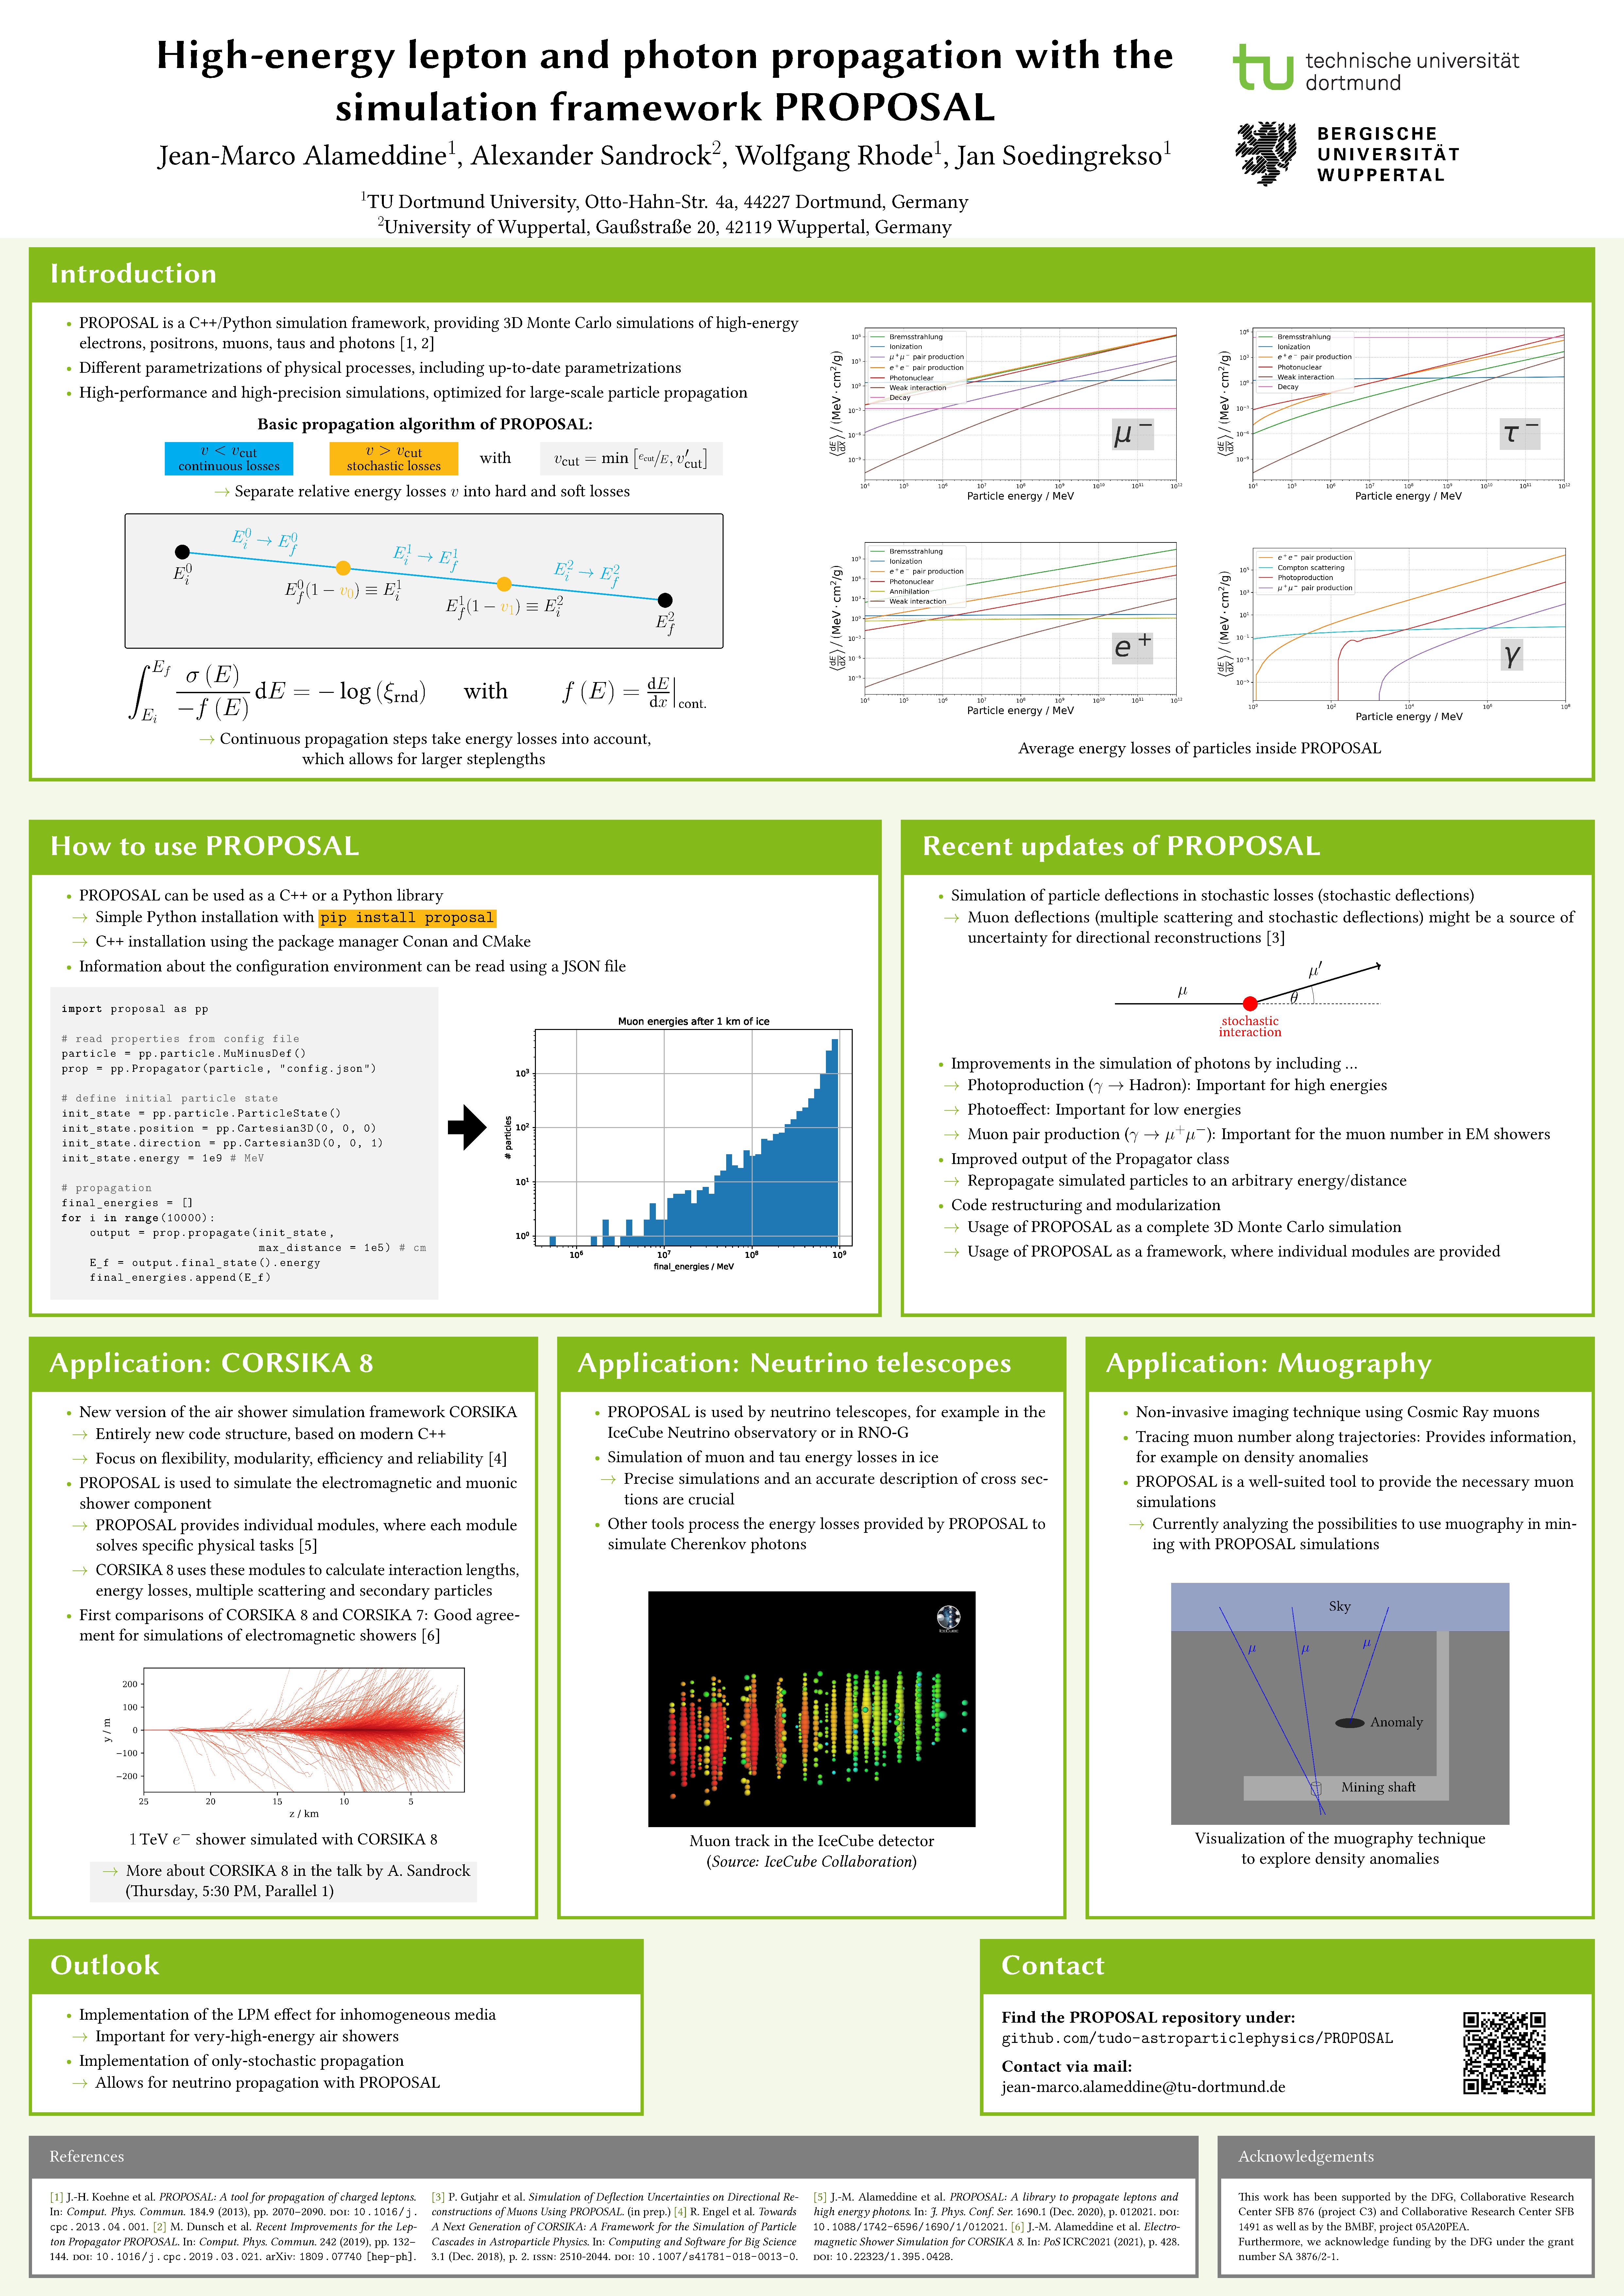
\includegraphics[clip, trim=0.5cm 78cm 0.5cm 12.5cm,width=\paperwidth]{../poster_print.pdf}}
\end{frame}
}


{
\setbeamertemplate{navigation symbols}{}
\begin{frame}[plain]
    \makebox[\linewidth]{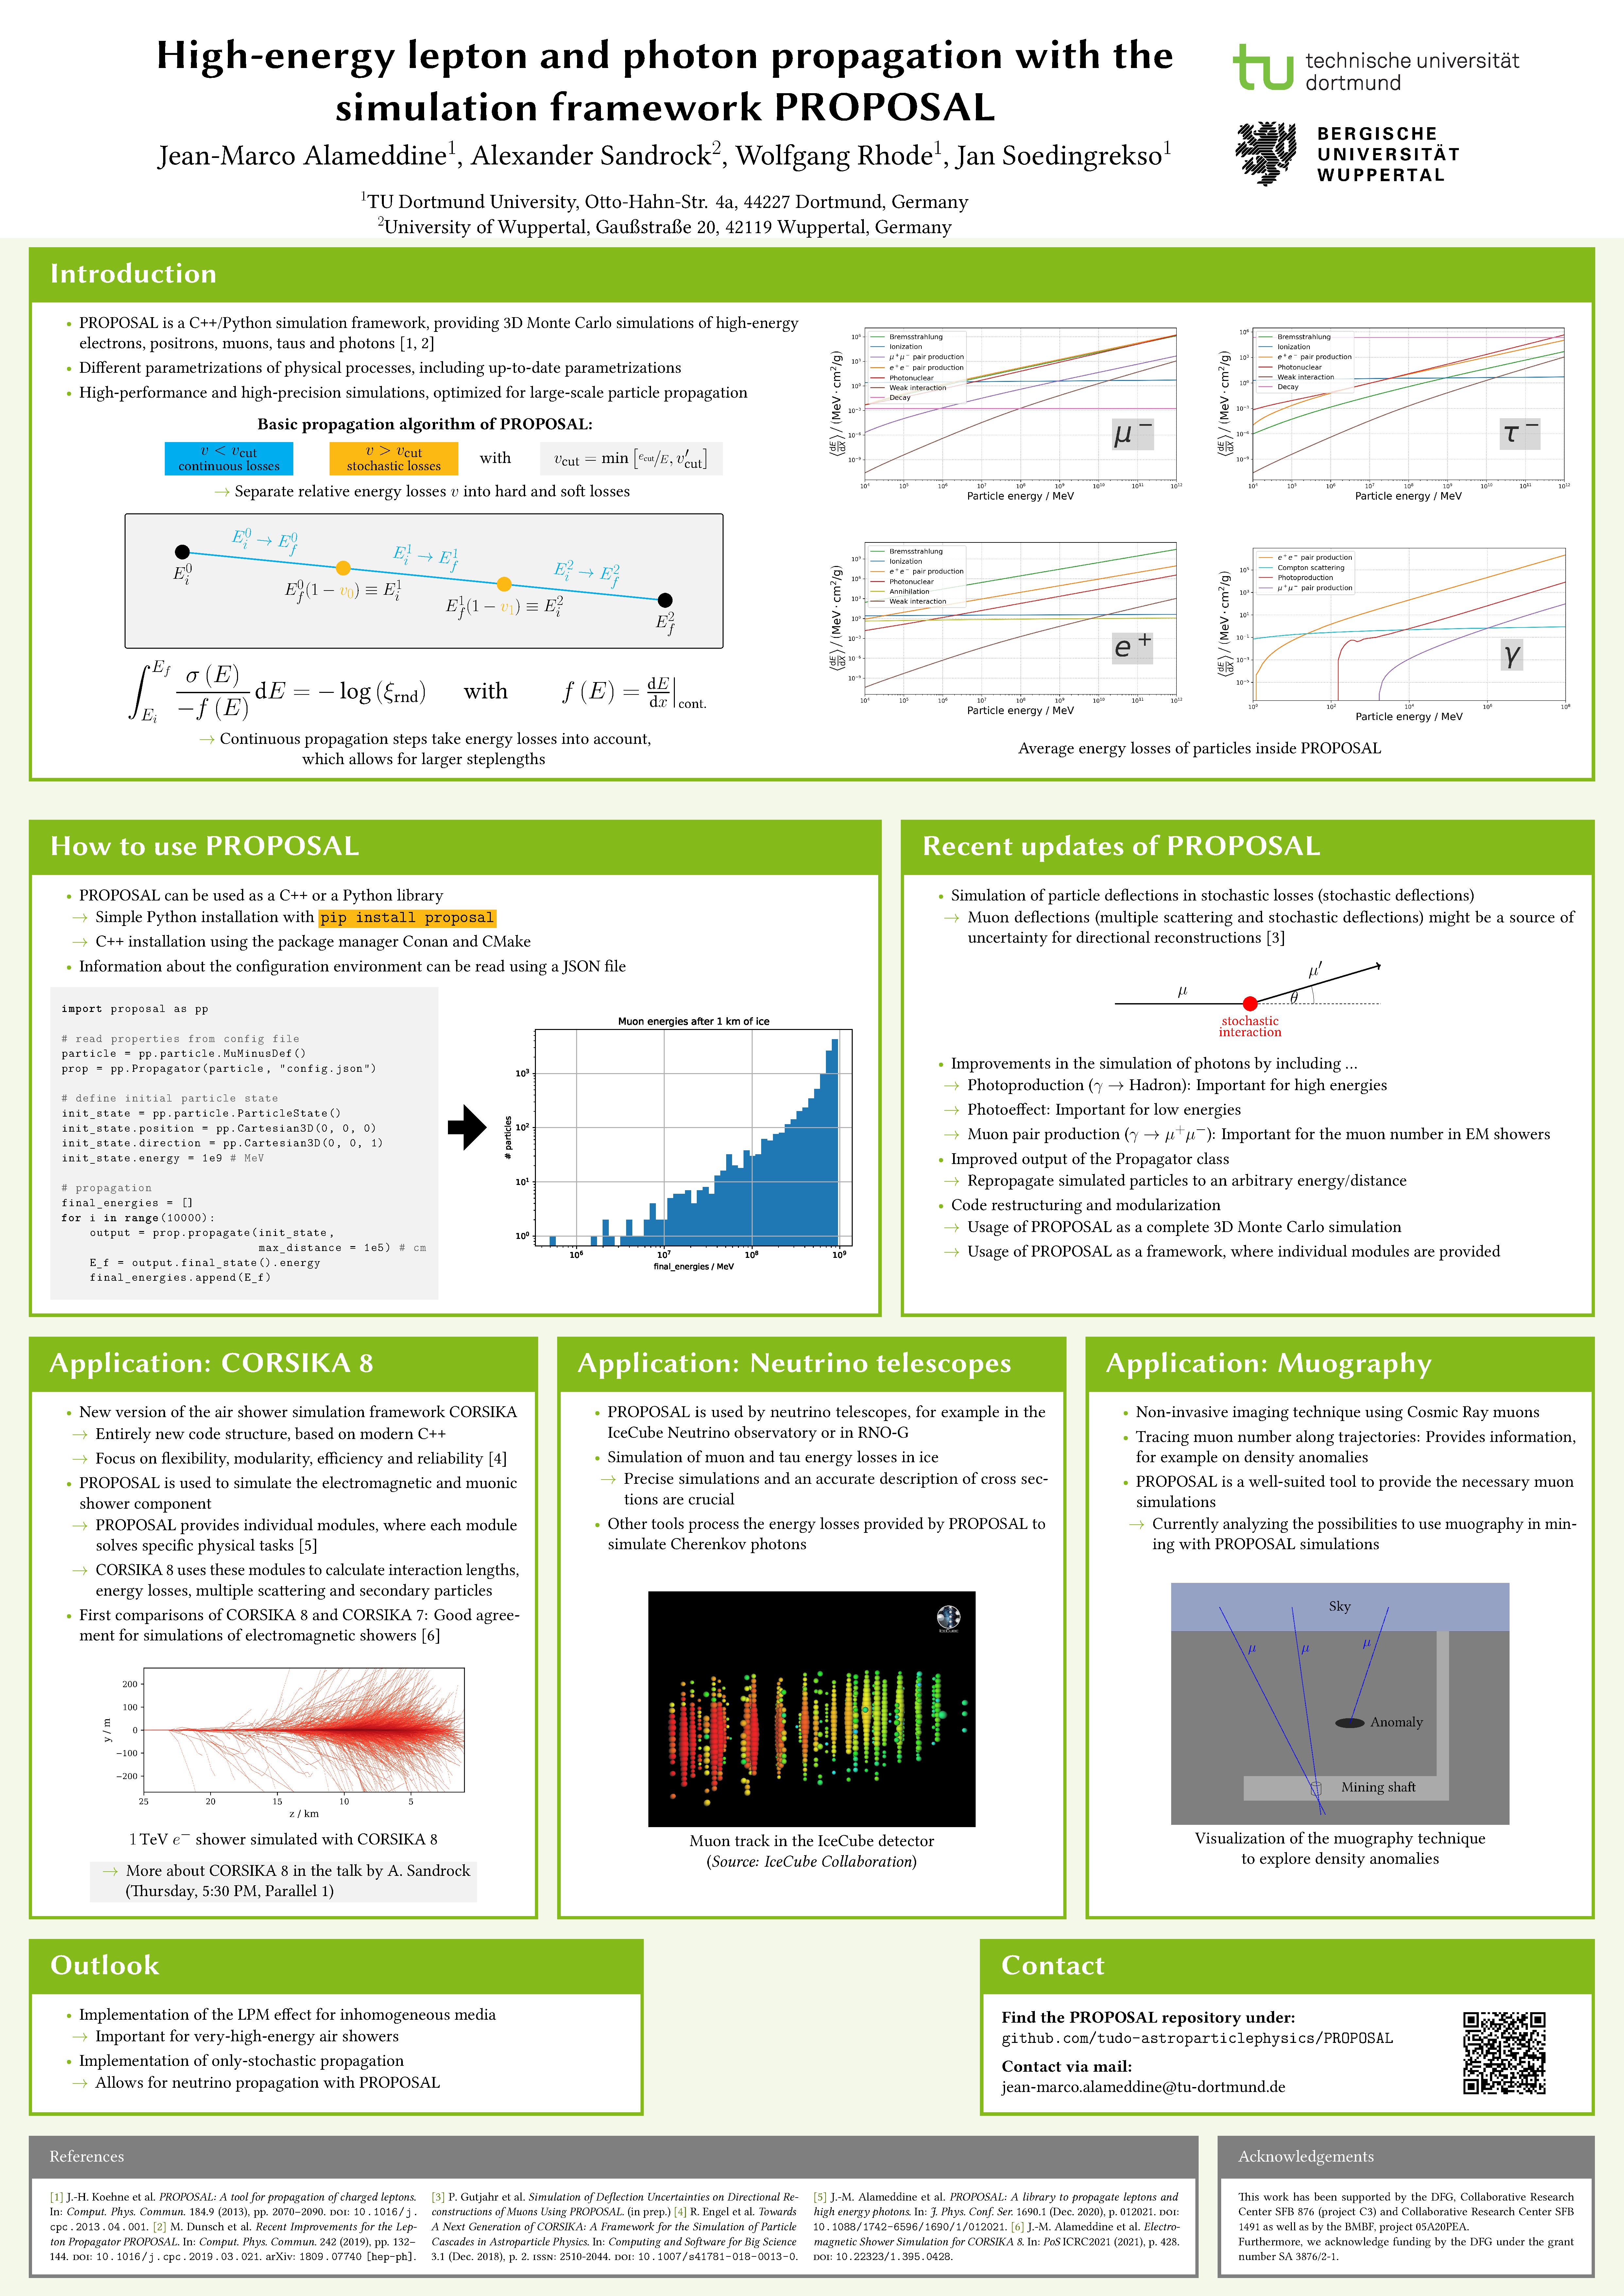
\includegraphics[clip, trim=0.5cm 50cm 0.5cm 41.5cm,width=\paperwidth]{../poster_print.pdf}}
\end{frame}
}

{
\setbeamertemplate{navigation symbols}{}
\begin{frame}[plain]
    \makebox[\linewidth]{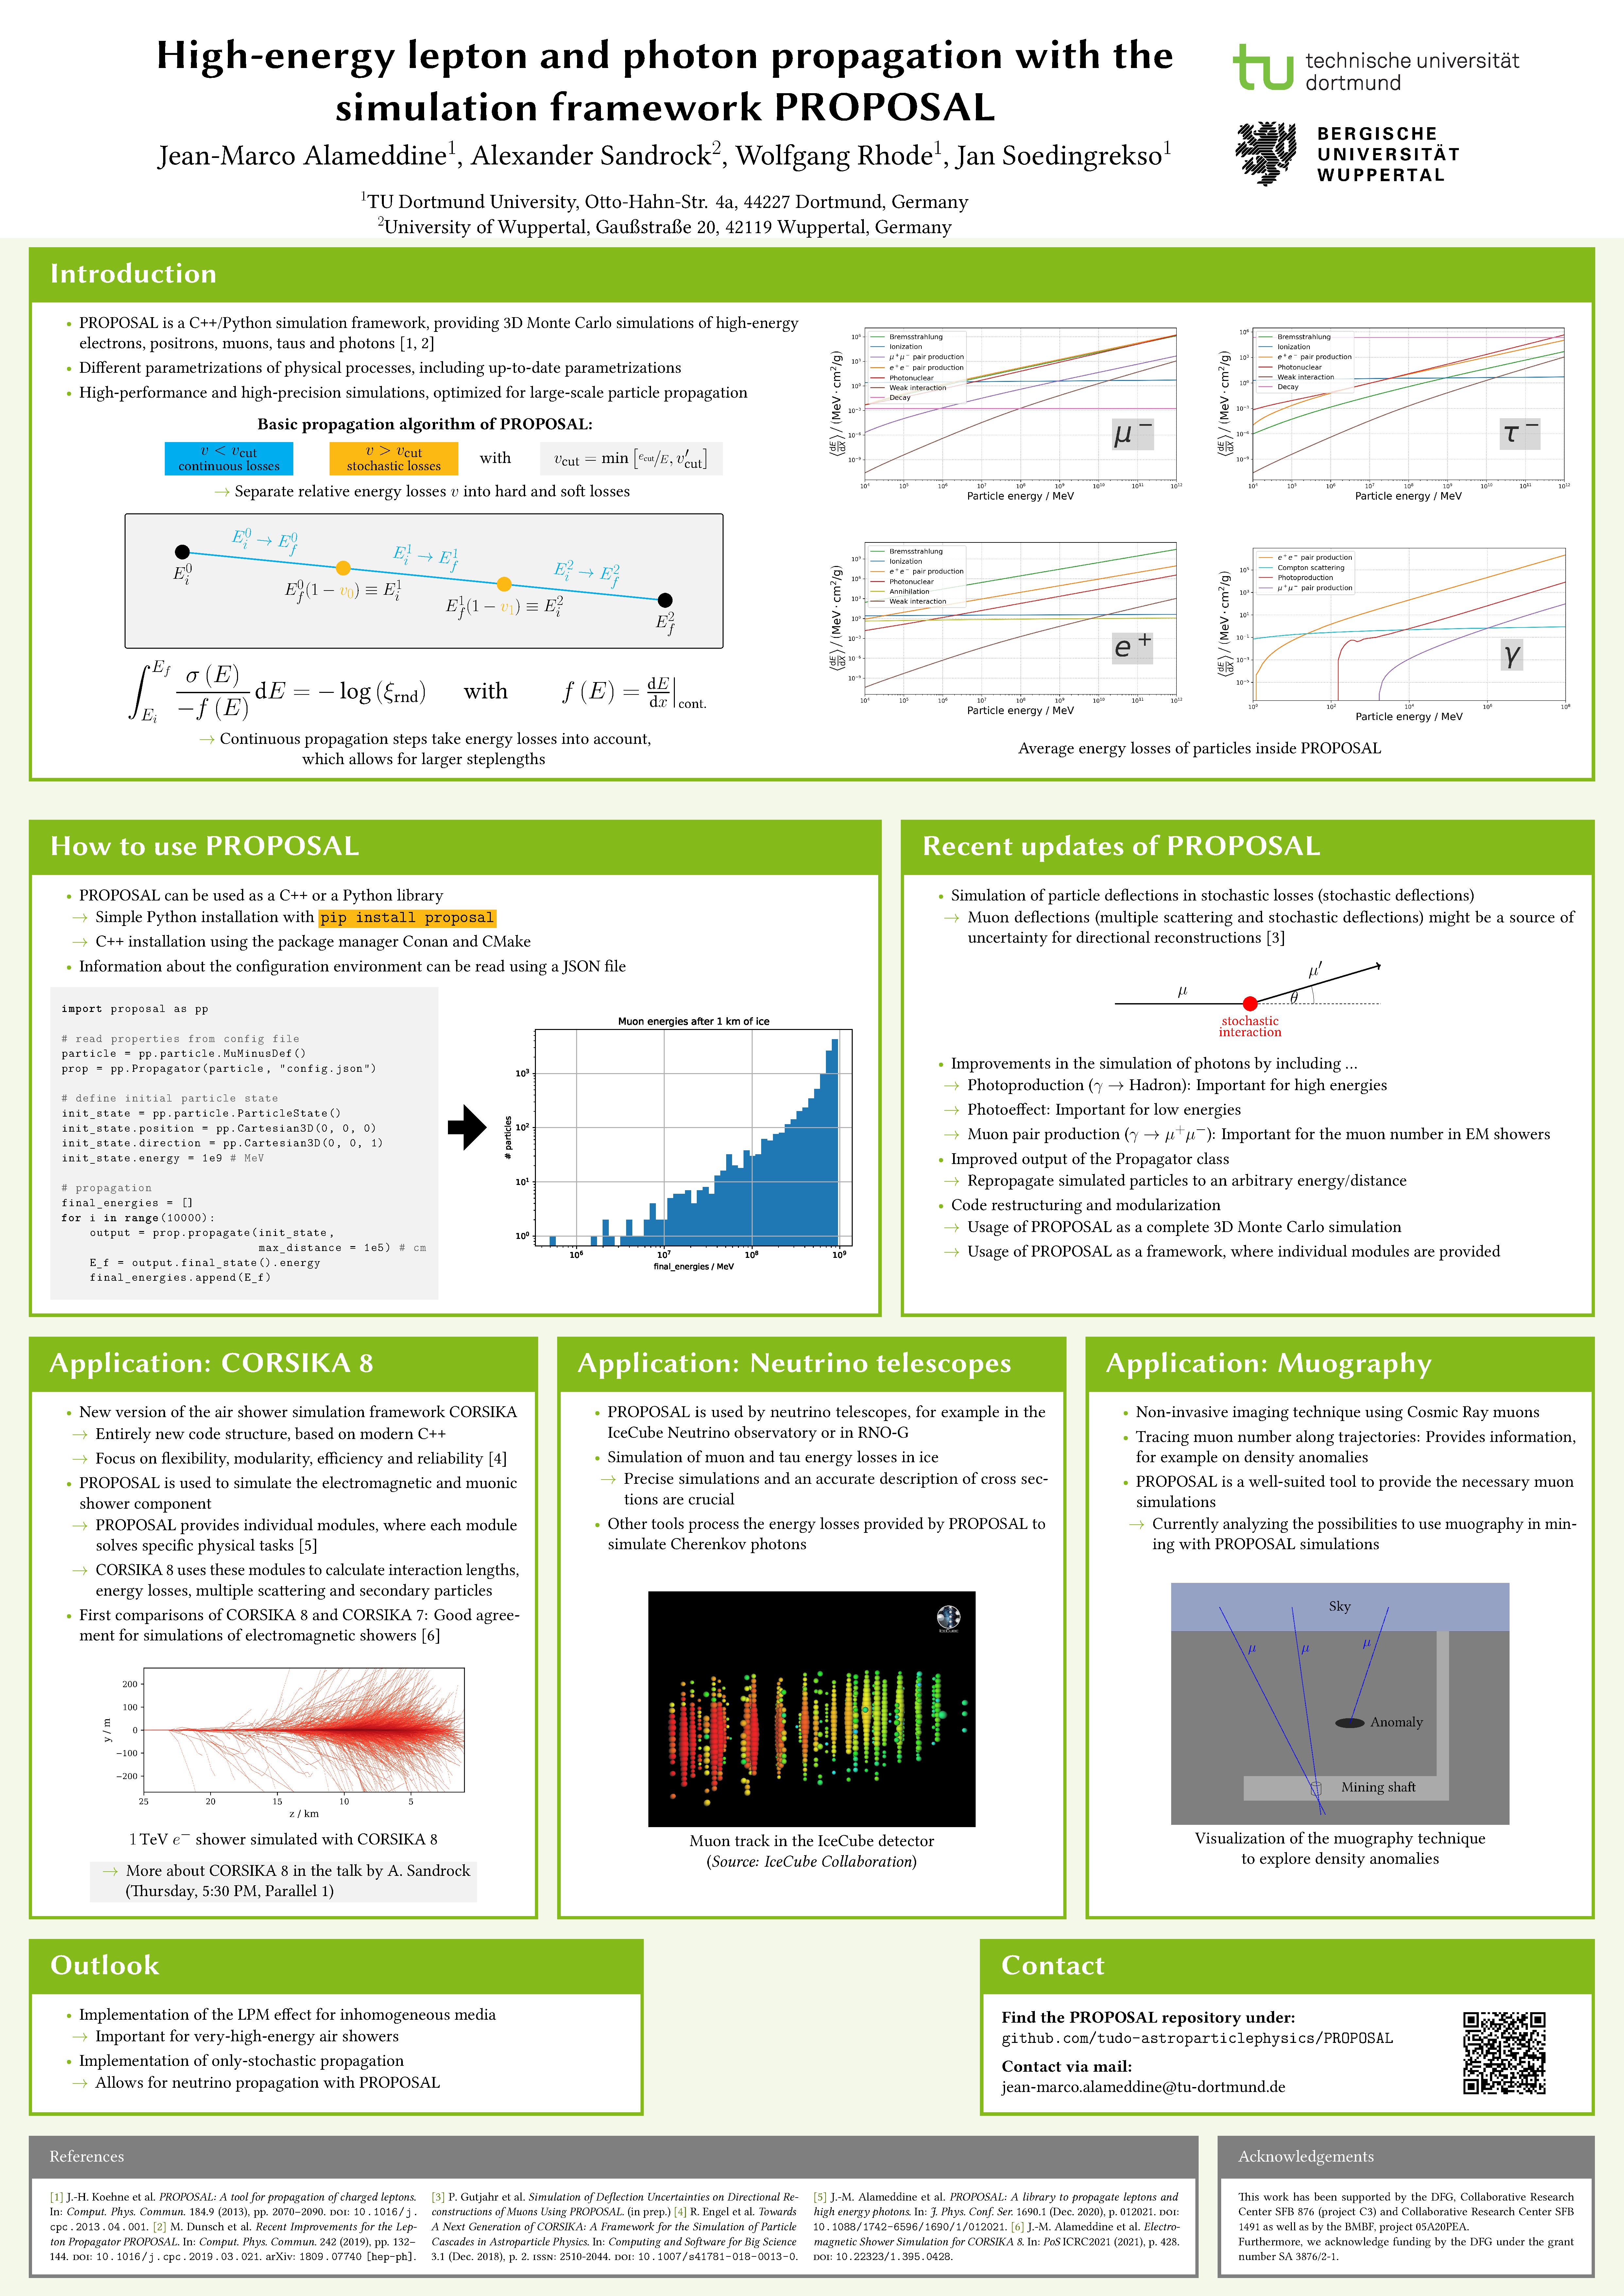
\includegraphics[clip, trim=0.5cm 19cm 0.5cm 68.5cm,width=\paperwidth]{../poster_print.pdf}}
\end{frame}
}


\end{document}
